

\subsection{Browser Fingerprinting APIs}
\label{sec:fp-apis}

We conduct an in-depth analysis in order to determine which browser features are associated with fingerprinting. We use this list of suspicious APIs in our measurements in Section~\ref{sec:analysis} to quantify \textit{fingerprintability}: the ratio of browser features in a browser version that are associated with fingerprinting techniques. We describe in the following how we conducted the list of suspicious browser features that are related to browser fingerprinting.

Our list of suspicious browser fingerprinting API contains a total of 313 JavaScript APIs. These APIs are considered suspicious because the purpose of using these API depends on the programmer who writes the source code. 
We call this list \textit{suspicious fingerprinting APIs} in this paper.
In Panopticlick's research~\cite{panopticlick}, browser fingerprinting is achieved through a combination of APIs that seem innocent, such as \texttt{Navigator.plugins}, \texttt{Navigator.userAgent}, and \texttt{Screen.colorDepth}. These APIs are designed with their original objectives. However, they are chosen to fingerprint browsers due to their alternative functionality in collecting information to narrow down the scope of visited users. Based on our approach taken to collect APIs, there is no way to determine whether the source code is doing browser fingerprinting without the acknowledgment of the writer of the code. 

We use two methods to assemble the list of fingerprinting APIs: literature review and experimental analysis. Literature review, the foundation of the API list, is composed of four core fingerprinting papers, Panopticlick~\cite{panopticlick}, AmIUnique~\cite{amiunique}, Hiding in the Crowd~\cite{hidinginthecrowd}, and FPDetective~\cite{fpdetective}. This analysis resulted in approximately 10\% of the list of suspicious fingerprinting APIs. Some of the APIs are directly mentioned in these papers and the others are modified to match standard APIs\footnote{\url{https://developer.mozilla.org/en-US/docs/Web/API}} with the same functionality. The concepts of Canvas, WebGL, Font fingerprinting are introduced among these APIs. These concepts lead to the next turn of investigation of papers which are Cookieless Monster~\cite{cookiemonster-SP13} and Pixel Perfect~\cite{mowery2012pixel}. This investigation does not bring more APIs but a direction to experimental analysis. 

The experimental analysis consists of two stages, collecting APIs by crawling websites and extracting suspicious APIs from the crawling data. In terms of data collecting, the workflow is the same as the one in VisibleV8~\cite{vv8-imc19}. A customized crawler was driven to visit all websites in the Easylist~\cite{Easylist} domain file that contains 13,241 domains. Then, the raw logs generated by VV8 were gathered and the VV8 post processor was applied to process the raw data. After removing duplicate and non-standard APIs, the APIs usage of 8,682 domains with 56,828 origins was collected. Non-standard APIs indicate ones that are not listed in the WebIDL~\cite{webidl} data package. In other words, VV8 and its post processor were adopted to aggregate and summarize standard JS API usage of the target domains.

While collecting APIs from the wild, the API suspicious list was extended through crawling on \url{panopticlick.eff.org}, \url{amiunique.org}, and \url{browserleaks.com} websites. These websites are explicitly marked as browser fingerprinting websites. Therefore, augmenting suspicious fingerprinting APIs among these websites is more efficient than a random walk on the enormous JS API pool.

The next step is to implement a manual analysis to check every API utilized by these three websites. First, we search for information and usage of an API on https://developer.mozilla.org/en-US/docs/Web/API. Then, determine whether an API fingerprints users based on the information the API conveys. That is to say, an API is classified as a suspicious fingerprinting API if it can provide the information to filter certain users out. For example, there are two users with distinct user agents. By calling Navigator.userAgent, the programmer should be able to distinguish between these two users. Navigator.userAgent can be recognized as a fingerprinting API in this case. The majority of suspicious fingerprinting APIs comes from the manual analysis and the idea of categorizing fingerprinting APIs is incited by browserleaks.com website. 

The last step is to manually search for more fingerprinting APIs with the keyword. Namely, in Canvas fingerprinting, most APIs include the ``Canvas'' or ``CanvasRendering''. A program was created to filtrate APIs that contain ``Canvas'' or ``CanvasRendering'' among APIs of 8k crawled domains. The same pattern also applies to BatteryManager, WebGLRenderingContext, and SpeechSynthesis. Meanwhile, the fingerprint2.js was reviewed to supplement the suspicious fingerprinting API list.  

There are limitations to the methods we used for constructing a suspicious fingerprinting API list. First and foremost, this list only provides a partial view of full fingerprinting APIs. To the best of our knowledge, there is no complete table of fingerprinting APIs and there could be research in this direction. The second limitation is during the manual analysis. There could be misconceptions between the API usage provided by Mozilla web APIs page and the way programmers exploit them. Lastly, part of JS APIs is filtered out by the VV8 post processor. This can be improved by using a larger set of WebIDL data or precisely use the aggregated raw APIs. 

We plan to make our list of fingerprinting APIs publicly available upon publication.

\subsubsection{Analyzing fingerprinting API presence in Browsers}
We wanted to answer two different questions regarding to browser fingerprinting in our paper. Are browsers becoming more fingerprintable as the time goes by? Can we also say that all browsers are fingerprintable?

Now that we have collected these fingerprinting APIs list, we try to examine different browser versions and see how many of these APIs are active in various browser versions.
We analyzed the presence of these APIs in every browser version in our analysis. For Chrome, we observe that Chrome 49, which is the youngest Chrome browser version in our analysis, has 139 fingerprinting APIs which is the smallest number among other versions.
On the other hand, Chrome 81, which is the latest Chrome browser in our analysis, has 274 fingerprinting APIs in it, which is the biggest number among other Chrome versions. So, it is obvious that Chrome is having more fingerprinting APIs in its newer versions and creating a unique fingerprint for the user is becoming easier in this browser. 
For Firefox, we figure out that the least number of APIs exist in Firefox 45 which is the youngest Firefox version in our study. The latest Firefox version which is Firefox 75 has 271 fingerprinting APIs in it but it is not the biggest number. Firefox 60 through 71 have 276 APIs which is the biggest number of APIs among other Firefox versions. It seems that fingerprinting APIs are being reduced in the latest versions of Firefox but newer versions are having much more features compared to the earlier versions.

In figure 6 we present the detailed information about presence of fingerprinting APIs in different browser versions.

\begin{figure*}[ht]
    \centering
    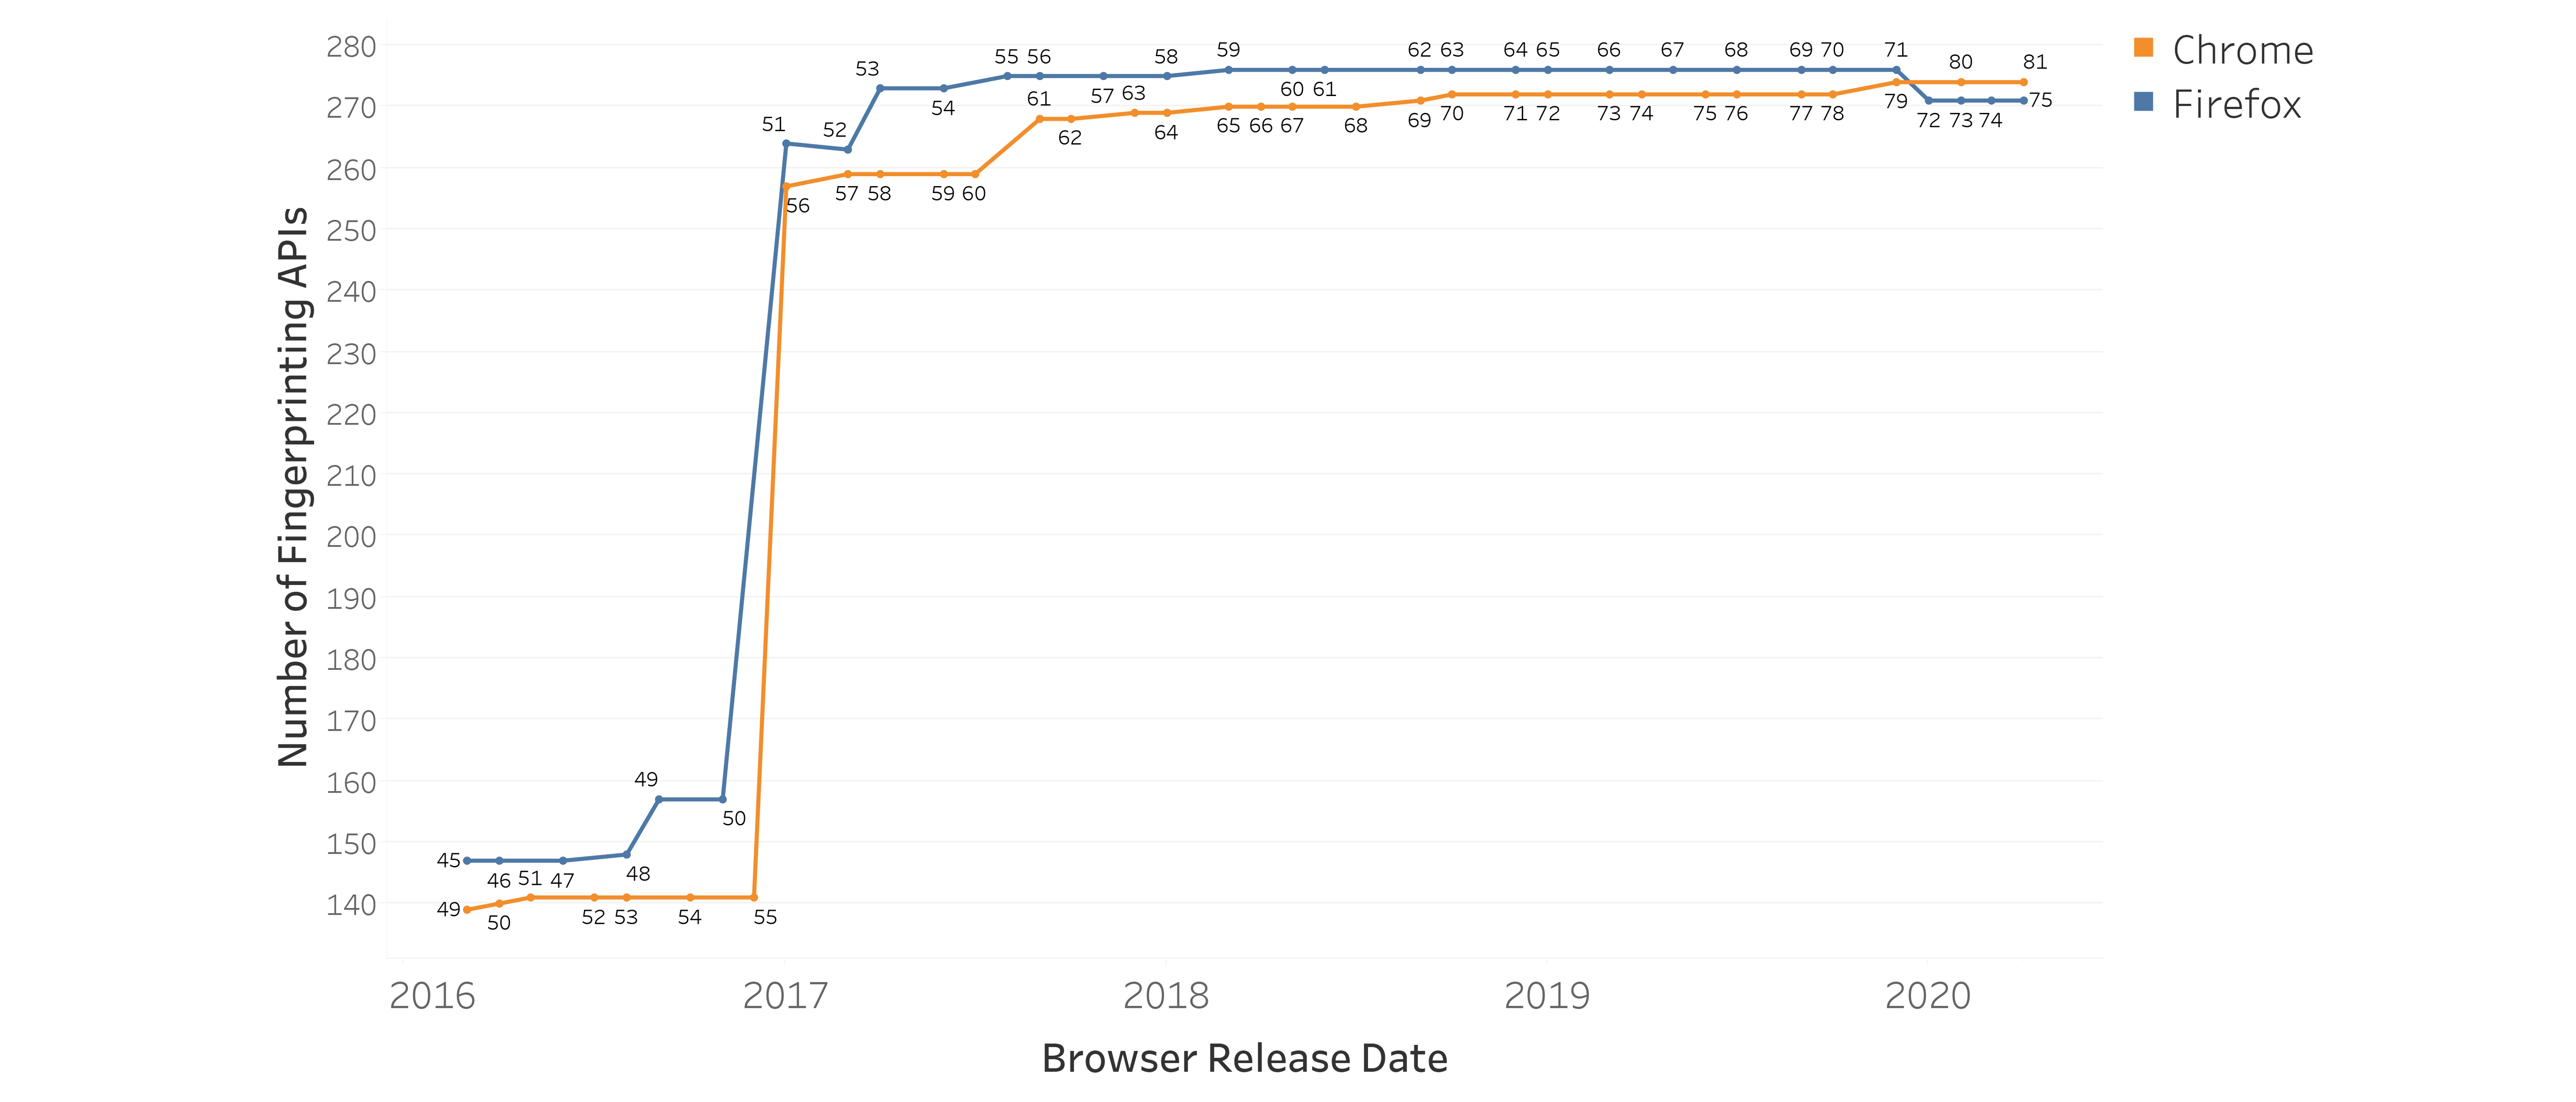
\includegraphics[width=\textwidth]{figures/Fingerprinting-APIs.png}
    \caption{Presence of Fingerprinting APIs among different browser versions. The orange line shows Google Chrome versions while the Blue line represents Firefox versions. The X-axis shows browser release date and the Y-Axis shows number of fingerprinting APIs.}
    \label{fig:fingerprint-apis}
\end{figure*}

\subsubsection{Unique Feature Set}
We created a feature set for each browser version that we had.
A feature set is a set of browser features that exist in a specific browser version.
After creating the feature set for each browser version in our study, we compared these sets to each other and realized that all of these sets are unique.
This means that there are no two browsers that have the same feature set which supplements our hypothesis that all browsers are fingerprintable. The presence of temporary and non-persistent features lead to this difference in feature sets among browsers. Vendors keep removing and adding features to their newer versions so that the feature set for each version is unique and different from the others.

One other observation of our study is that vendors especially Google Chrome are adding lots of features to their newer versions but they do not remove features as much as they add. We define a set called unique feature set as the set of features that make a specific browser version unique; either by existing in the feature set of that browser or by not being in the feature set. We generate the unique feature set for every browser in our study and see that this set is getting smaller over time in newer versions. Thus, we can say that the feature set for newer browsers is becoming more similar and they have much more intersection with each other compared to the older ones. So the feature set for browsers is converging and we are tending to the homogeneity of browser features. 

